\documentclass[british,titlepage]{ntnuthesis}

\title{An NTNU Thesis \LaTeX{} Document Class}
\shorttitle{An NTNU Thesis Document Class}
\author{Community of Practice in Computer Science Education at NTNU}
\shortauthor{CoPCSE$@$NTNU}
\date{CC-BY \ntnuthesisdate}

\addbibresource{thesis.bib}


% From https://www.overleaf.com/learn/latex/Glossaries

\makeglossaries % Prepare for adding glossary entries


\newglossaryentry{latex}
{
        name=latex,
        description={Is a mark up language specially suited for
scientific documents}
}

\newglossaryentry{bibliography}
{
        name=bibliography,
        plural=bibliographies,
        description={A list of the books referred to in a scholarly work,
typically printed as an appendix}
}

\newglossaryentry{maths}
{
    name=mathematics,
    description={Mathematics is what mathematicians do}
}

% Words to define
%scrum
%frontend
%backend
%api
%dataset
%kanban
%biometric
%REST / RESTful
%sprint
%use case
%Github
%repository
%React.js
%Node.js
%Axios
%web framework? Explain what it is
%Docker
%Containerization / containers
%dockerfiles
%biometric
%Telegram

% --------------------
% ----- Acronyms -----
% --------------------
\setglossarypreamble[acronym]{The page number after an acronym refers to the first time it is used in the thesis.}
\newacronym{api}{API}{Application Programming Interface}
\newacronym{ai}{AI}{artificial intelligence}
\newacronym{cie}{CIE}{International Commission on Illumination}
\newacronym{cnn}{CNN}{Convolutional Neural Network}
\newacronym{covid19}{COVID-19}{Coronavirus disease 2019}
%\newacronym{csv}{CSV}{Comma-separated values}
\newacronym{cvd}{CVD}{Colour Vision Deficiency}
\newacronym{dom}{DOM}{Document Object Model}
\newacronym{xml}{XML}{Extensible Markup Language}
\newacronym{xhtml}{XHTML}{Extensible HyperText Markup Language}
\newacronym{xp}{XP}{Extreme Programming}
\newacronym{fiqm}{FIQM}{Face Image Quality Metric}
\newacronym{fiqa}{FIQA}{Face Image Quality Assessment}
\newacronym{fr}{FR}{Face Recognition}
\newacronym{gdpr}{GDPR}{General Data Protection Regulation}
\newacronym{html}{HTML}{HyperText Markup Language}
\newacronym{http}{HTTP}{Hypertext Transfer Protocol}
\newacronym{icao}{ICAO}{International Civil Aviation Organization}
\newacronym{iec}{IEC}{International Electrotechnical Commission}
\newacronym{iso}{ISO}{International Organization for Standardization}
\newacronym{json}{JSON}{JavaScript Object Notation}
\newacronym{mrtd}{MRTD}{Machine Readable Travel Documents}
\newacronym{mvc}{MVC}{Model-View-Controller}
\newacronym{mtcnn}{MTCNN}{Multitask Cascaded Convolutional Networks}
\newacronym{ntnu}{NTNU}{Norwegian University of Science and Technology}
%\newacronym{ux}{UX}{User Experience}
%\newacronym{ui}{UI}{User Interface}


 % add glossary and acronym lists before document

\begin{document}

\chapter*{Abstract}

The performance of face recognition systems are dependent on images used for training and analysis. There are metrics that automatically can calculate the quality of the images. In this project we have evaluated two face image quality metrics provided by Mobai. The project consisted of creating a web application that automates the process of evaluating datasets and that can easily add new FIQMs into the application. We are also comparing the scores provided by the FIQMs with human assessments by arranging a subjective experiment to collect ground truth data. 


The performance of face recognition systems are dependent on images used for training and analysis. There are metrics that automatically can calculate the quality of images. In this project we have evaluated two face image quality metrics provided by Mobai. The project consisted of creating a web application that evaluates images by the use of different Face Imaqe Quality Metrics (FIQM). We have also conducted a subjective experiment to collect ground truth data on three datasets Mobai gave us and compared them with the scores from the FIQMs to see the correlation. Further, we have expanded the task by creating our own dataset consisting of new aspects and distortions, and conducted a new subjective experiment. The subjective results from this dataset has then been used to correlate with the two FIQMs.

\chapter*{Sammendrag}
Ytelsen på ansiktgjenkjenningssystmer er avhengig av kvaliteten på bildene for å kunne teste og trene disse systemene. For å automatisk vurdere kvaliteten på ansiktsbilder blir Face Image Quality Metrics (FIQMs) benyttet. Slike kvalitetsmetrikker gir objektive resultater som korresponderer med hvor synlig ansiktet i et bilde er. I dette prosjektet introduserer vi en webapplikasjon som regner ut slike objektive resultater med to moderne FIQMs. For å vurdere nøyaktigheten på disse metrikkene, samlet vi inn subjektive data fra eksperter og ikke-eksperter på tre forskjellige dataset. Vi samlet også inn et nytt dataset med ansiktsbilder som vi mener er overlegent i forhold til andre nåværende dataset. Denne overlegenheten er med tanke på antall bilder, type forvregninger bildene er påvirket av og hvordan bildet er tatt (bilder med ansiktsmasker og bilder med skrå vinkler). Resultatene viser at de objektive resultatene regnet ut av de to kvalitetsmetrikkene har lav korrelasjon med de subjektive resultatene samlet inn via subjektive eksperimenter. 


\tableofcontents
\listoffigures
\listoftables
\lstlistoflistings

\printglossary[type=\acronymtype] % Print acronyms
\printglossary                    % Print glossary

\chapter{Introduction}
\label{chap:Intro}

\section{Background}
\label{section:background}
Mobai is a spin off company from the research developed in the Norwegian Biometrics Laboratory at the \acrfull{ntnu}. They provide solutions for facial recognition, biometrical attack detection and face morph detection. To create models for detection of biometrical attributes, artificial intelligence \acrshort{ai} and machine learning are essential tools for Mobai. In addition to the models, having access to appropriate datasets plays a crucial role in training and developing new models. An important focus of Mobai is using different \acrlong{fiqm}s (\acrshort{fiqm}s) to determine the quality of facial images in a dataset. In order to train models, quickly assess several datasets or create new datasets, it is important to know the quality of facial images. Therefore, Mobai now aims to develop an application that automates this process. 

\section{Subject Area}
Digital image processing is a rapidly growing field within the world of engineering and computer science. A great amount of research has been done in this field of study, paving the way for multimedia systems to become one of the pillars of the modern information society. Digital image processing is used in a variety of technologies, including face detection and face recognition which itself could be categorized under the broader field of patter recognition. Digitalization has drastically changed peoples everyday lives over the last decade, and with that change, biometrics has become more relevant and important than ever. 

Solutions such as face recognition, presentation attack detection and face morph detection all heavily rely on the quality of the facial images used for machine learning training. The quality of facial images are dependent on several factors which FIQMs have learned trough artificial intelligence and machine learning. FIQMs' performance can be measured by comparing the quality scores with human assessment. This thesis is mainly focused on Face Image Quality Assessment (\acrshort{fiqa}) which plays a key role in improving the accuracy of face recognition systems. 

\section{Task Description}
\label{sec:TaskD}
This bachelor project can be divided into two main parts, a programming part (mainly Chapter \ref{chap:objective}) and a research part (mainly Chapter \ref{chap:subjective}).

\subsection*{Programming}
The programming part involves the creation of an application that uses two FIQMs provided by Mobai for evaluating the quality of facial images. The application will create a report which contains the FIQM calculations in the set of images. The key functionalities of the application expected from Mobai are: 
\begin{itemize}
    \item The user should be able to read/select images from a local machine.
    \item The user should be able to upload images to a directory.
    \item The user should be able to execute the two FIQMs on the uploaded images.
    \item The user should be able to display the results from the FIQMs. 
\end{itemize}

\subsection*{Research}
The research part consists of conducting a subjective experiment. The subjective experiment involves collecting ground truth data by having subjects evaluate the quality of facial images from a dataset based on certain criteria. During the experiment, observers will be shown different facial images of varying quality and asked to label the images into predefined categories. The subjective results will then be used to compare with the objective results from the FIQMs. By comparing the subjective results from the experiment with the objective measure calculated by FIQMs we are then able to evaluate the performance of FIQMs. 

\section{Delimitation}
\label{sec:delimit}
In this project, our task was not solely made up of pure programming. Fortunately, the subject field we were working within allowed research which we found to be a great experience in the final step of our bachelor studies. As an example, facial images used for research in the field of face quality assessment and face recognition were usually taken from a straight angle with little to no tilting of the camera lens. After a literature review it was evident that studies addressing camera tilting was very limited. With the ongoing pandemic, wearing face masks in public has become a habit. Even though wearing a mask is a new aspect of our daily lives, the performance of FIQMs on images which show a subject wearing a face mask has not yet been studied. In that case, we wanted to assess the performance of the FIQMs on face mask images. For the mentioned reasons, the bachelor group proposed the collection of a new dataset which Mobai supported the initiative. The mentioned dataset will not only be used by Mobai in their studies but can also be used by the bachelor group. Further information about the collected dataset is provided in Section \ref{sec:ownData}. Finally we should point out that with the exception of our dataset, all FIQMs and datasets were provided to the bachelor group by Mobai. 

\section{Target Groups}
\label{sec:TargetGroups}
In general, this project is targeted towards two groups, Mobai and the readers of the thesis. 

\subsection{Users of the Web Application}
The web application will be used by employees at Mobai to evaluate the performance of the FIQMs on different datasets. Based on the Non Disclosure Agreement (NDA) signed by the bachelor group (Appendix \ref{app:project-agreements}), because of possible competitive companies neither the source code or the application should be distributed to others except Mobai.

\subsection{Thesis Readers}
The target group for the bachelor thesis are people who need insight in how we did the project from a developer point of view as well as a scientific point of view. This includes but is not limited to our thesis supervisor, client and fellow students with similar background that can be interested in reading the thesis.

\section{The Team}
In this section we will introduce the members in our team. Here we look at their interests, responsibilities and their academic backgrounds. 

\subsection{The Members}

\subsubsection*{Hans Petter}
Hans Petter is a computer engineer who is interested in mathematics and artificial intelligence. He is interested in Python programming and was therefore one of the main developers of the backend. Hans Petter had the main responsibility for implementing \acrshort{api}s to the frontend. He also helped out the other team members whenever there were any API errors connecting Flask to React or general Python problems. In addition to the application task, Hans Petter collected the data from the subjective experiment to make it workable. 

\subsubsection*{Walid}
Walid has prior knowledge with artificial intelligence and finds topics that mix statistics and mathematics with artificial intelligence interesting. Throughout the project, Walid was mainly involved in the creation of the backend logic with Hans Petter. In particular, he developed API endpoints used by the frontend. 

\subsection*{Julian}
Julian is a computer engineer with an interest in programming, mathematics and artificial intelligence. His background consists of different subjects regarding programming, mathematics, software security and application development. Julian's main responsibility was creating the frontend of the application and handling the data received by the backend. 

\subsubsection*{Kjetil}
Kjetil is a developer with an interest in front end web-development, JavaScript and Python programming. Due to his background and interests, his main responsibility was to work with the frontend and help with the backend development. 


\subsection{Academic Background}
\label{section:academic background}
All group members are studying for a bachelor´s degree in computer engineering, hence our academic backgrounds are closely similar. However, during the fifth semester, we all chose different subjects. Hans Petter and Walid both chose \textit{artificial intelligence}, \textit{software design} and \textit{calculus 3}. Julian had the elective subjects \textit{application development}, \textit{software security} and \textit{calculus 3}, while Kjetil studied the subjects: \textit{ergonomics in digital media}, \textit{infrastructure as code} and \textit{application development}. 

Throughout our bachelor´s program we have acquired a solid foundation when it comes to the software development process and scientific thinking by finishing courses like \textit{software engineering}, \textit{algorithmic methods}, \textit{operating systems}, \textit{scientific computing}, \textit{calculus} and \textit{physics}. The compulsory courses we finished helped us see different approaches to the same problem. There will always be several ways to approach a task and a bachelor´s degree in computer engineering has cemented that statement. Our prior knowledge made it easier to understand and process the main concepts of the new topics we had to learn. 

During this semester, we have acquired more knowledge and built on our foundation. We had to perform research on specific topics in backend and frontend programming, as these were topics we were unfamiliar with. More specifically, the part of connecting the frontend to the backend by using API calls, was something we had never done before. In addition to that, a high amount of time was also spent on learning how to conduct and perform scientific experiments in a way that satisfies both \acrfull{gdpr} and the relevant \acrshort{iso}-standards.  

\section{Why Did We Choose This Task?}
Although stationed in Gjøvik the group had never heard of Mobai or what they do. Their task description seemed interesting, and we were early to contact them. Already at the first meeting, before any bachelor tasks were selected, we got a very positive impression. The participants from Mobai were very curious and enthusiastic. They had clear ideas and suggestions on how we could approach the task. After this meeting, the bachelor thesis choice became an easy decision. 

A reason why we chose this task was the field of work. All group members were interested in machine learning and artificial intelligence. Therefore, we saw the topic as a perfect opportunity to have a hands on experience working in this field. Another reason for our choice was the width of the project. We felt that we could use experiences and knowledge learned throughout the bachelor courses in this work. We had to combine math, statistics and programming with research, which given our bachelor's program suited us well. This kind of scope was complex, but manageable, and challenged us in several ways in terms of coding and research. We were motivated by the fact that Mobai expected us to create an application that they would utilize in addition to creating a subjective experiment.   

\subsection{Roles}
\label{subsec:roles}
Our project work areas were mainly divided into two categories: research and programming. While studying FIQMs, the subjective assessment and the creation of a subjective experiment which can be seen as research were done collectively to ensure equal professional foundation. When it came to the programming part, each group member were delegated responsibility more individually. However, due to the nature of the work, we had to closely collaborate with each other with backend and frontend because its dependency. During the project, the following roles were assigned to each group member:
\begin{itemize}
    \item Kjetil Grosberghaugen was scrum master and developer. His main responsibility was frontend, written in React.js. As a scrum master he ensured the development process flew evenly and led sprint meetings.
    \item Julian Nyland Skattum was a developer with main responsibility in frontend. He was also responsible for programming language choices as well as the overall application appearance. 
    \item Hans Petter Fauchald Taralrud was a developer with main responsibility\\ in backend. 
    \item Walid Demloj was a developer with main responsibility in backend. 
\end{itemize}

Every member were participating in the full stack application despite their area of responsibility. The reason for having individual responsibilities was to easily maintain that the requirements were met. The group members had joint responsibility for the project plan (see Appendix \ref{app:project-plan}) and thesis as well as completing tasks according to the created requirements. 

Seyed Ali Amirshahi was our supervisor. The project group had scheduled meetings every Monday at 12:00. Ali's role in the project was to guide us throughout the project. He would evaluate the project plan, thesis and answer professional questions. Summaries of the meetings with Ali be found in Appendix \ref{appendix:supervisor}.

Kjartan Mikkelsen started as the product owner, but after about three months in the process, he left the company. Our new product owner and contact was Guoqiang Li. He expressed Mobai's vision and wishes during the project. We also got technical assistance from other employees at Mobai. Summaries of the meetings with Mobai can be found in Appendix \ref{appendix:Mobai}.

\subsection{Decision Making}
The group decided to go for a collaborative decision-making \cite{GroupDecisionMaking} approach when making choices throughout the project. Decisions like frontend and backend environment and experiment platform were decided collectively with knowledge and experience in mind. A touch of prior knowledge benefited our project, so we did not need to learn everything from scratch. Making choices in groups led to a comfortable team atmosphere with a good relationship between each team member. The decentralization of decision responsibilities made it easier to contribute in the decision making, because possible failures would be shared in the group. However, if a discussion had reached an impasse, the group leader had the final say. Choices related to project work were brought up in the daily scrum meetings, as they offered frequent changes as well as a cordial environment to give feedback and improvements. Choices related to project organization was arranged in the sprint retrospective meetings, every other week. 


\section{Thesis Structure}
It is important to emphasize that this thesis is atypical. As almost every bachelor task include reporting the development process, our thesis adds an extra dimension in terms of research. The subjective part requires thorough research to be able to correctly compare with the results provided by the application. All this are reflected in the way we structured our thesis. 
We have chosen to structure the thesis as follows: in Chapter \ref{chap:Specification}, we are discussing our choice of development methodology. We look at pros and cons for the methodology, address other possible development methods and elaborate the current development layout. Following the chosen development approach is an in-depth risk analysis. Chapter \ref{chap:FQA} is an important part of the thesis. Here we define some of the most essential concepts used in the project. We describe the definition of a good facial image in face recognition as well as introducing the FIQMs used in the application. Next, in Chapter \ref{chap:objective} we will look at how the face image metric application has been implemented and the reasoning behind our choices. In Chapter \ref{chap:subjective} we go through the process of conducting a subjective experiment to gather ground truth data. We also introduce the datasets used in the experiment and explain our own dataset creation. 
Both the objective assessment and subjective experiments are merged together in the results Chapter \ref{chap:Results}, where their results are compared. Following the results, we can conclude the FIQMs strengths and weaknesses based on their correlation with the subjective scores. In the conclusion Chapter \ref{chap:Conclusion} we conclude the results and introduce further work based on our research. The reasoning behind this project structure is mainly to provide the thesis readers a clear overview and a sequential story. Since the project's contents of the work are split, it is meaningful to describe the workload in separate chapters. 
\chapter{Theory}
\label{chap:usage}

\section{What is a good image?}
\label{sec:setup}
Throughout this thesis we will mention the word quality several times. While some people already have a good understanding of what the word means, some confusion may arise. 

Within the standard image quality assessment field, quality´s definition is straight forward and is what most people think about when hearing the word. Ordinary people and people working with images will for the most part think about the image resolution as the most important characteristic that defines image quality. An excellent image of a face with this definition would have high resolution and sharp focus.   

However Mobai´s and our definition differs from the usual way image quality is defined. Our emphasis lies not with the image resolution itself, but rather how well the face is visible. There are several aspects that heavily affect the quality of facial images with respect to biometric systems performance. These aspects are presented and discussed in two important papers: 

\begin{itemize}
    \item ISO/IEC TR 29794-5:2010: Information technology — Biometric sample quality — Part 5: Face image data. \footnote{\url{https://www.iso.org/standard/50912.html}}
    \item ICAO Doc 9303 Part 3: Specifications Common to all MRTDs. \footnote{\url{https://www.icao.int/publications/Documents/9303_p3_cons_en.pdf}}
\end{itemize}

The quality specific aspects of facial images presented in the two standards are what defines the quality in our thesis. The different quality factors are:  

\begin{itemize}
    \item Image properties like the size of the image or its resolution.
    \item Image appearance characteristics like the exposure or noise.
    \item Scenery characteristics like lighting or background.
    \item Characteristics like the consistency between the skin colour on the image and the skin colour of the subject.
    \item Complete or partial face coverings.
    \begin{itemize}
        \item Glasses fully covering the eyes.
        \item Any type of head coverings.
    \end{itemize}
    \item The behaviour of the subject.
    \begin{itemize}
        \item Closed or open eyes.
        \item Closed or open mouth.
        \item Any kind of expression, e.g. smiling or neutral.
        \item Head pose, e.g. frontal or rotated in any direction.
    \end{itemize}
\end{itemize}

The above mentioned aspects all affect the quality of the facial image to some degree. What we consider an excellent facial image is similar to a standard passport image with the following characteristics: 
\begin{itemize}
    \item Open and visible eyes.
    \item No dark tinted glasses. 
    \item Neutral or little to none facial expression.
    \item Neutral head pose.
    \item No garments covering the face.
    \item Clean background.
    \item Neither too dark or too light.
    \item Photo taken neither too close or too far away.
    \item Face is centered.
\end{itemize}

The characteristics will affect the quality in a good or bad way. If all the bullet points above are true, the quality of the facial image is near perfect. An image of a half-covered or missing face will negatively affect the quality, even though the image resolution itself may be impeccable. 

\begin{figure}[h]
\centering
    \subfloat[Excellent facial image]
        {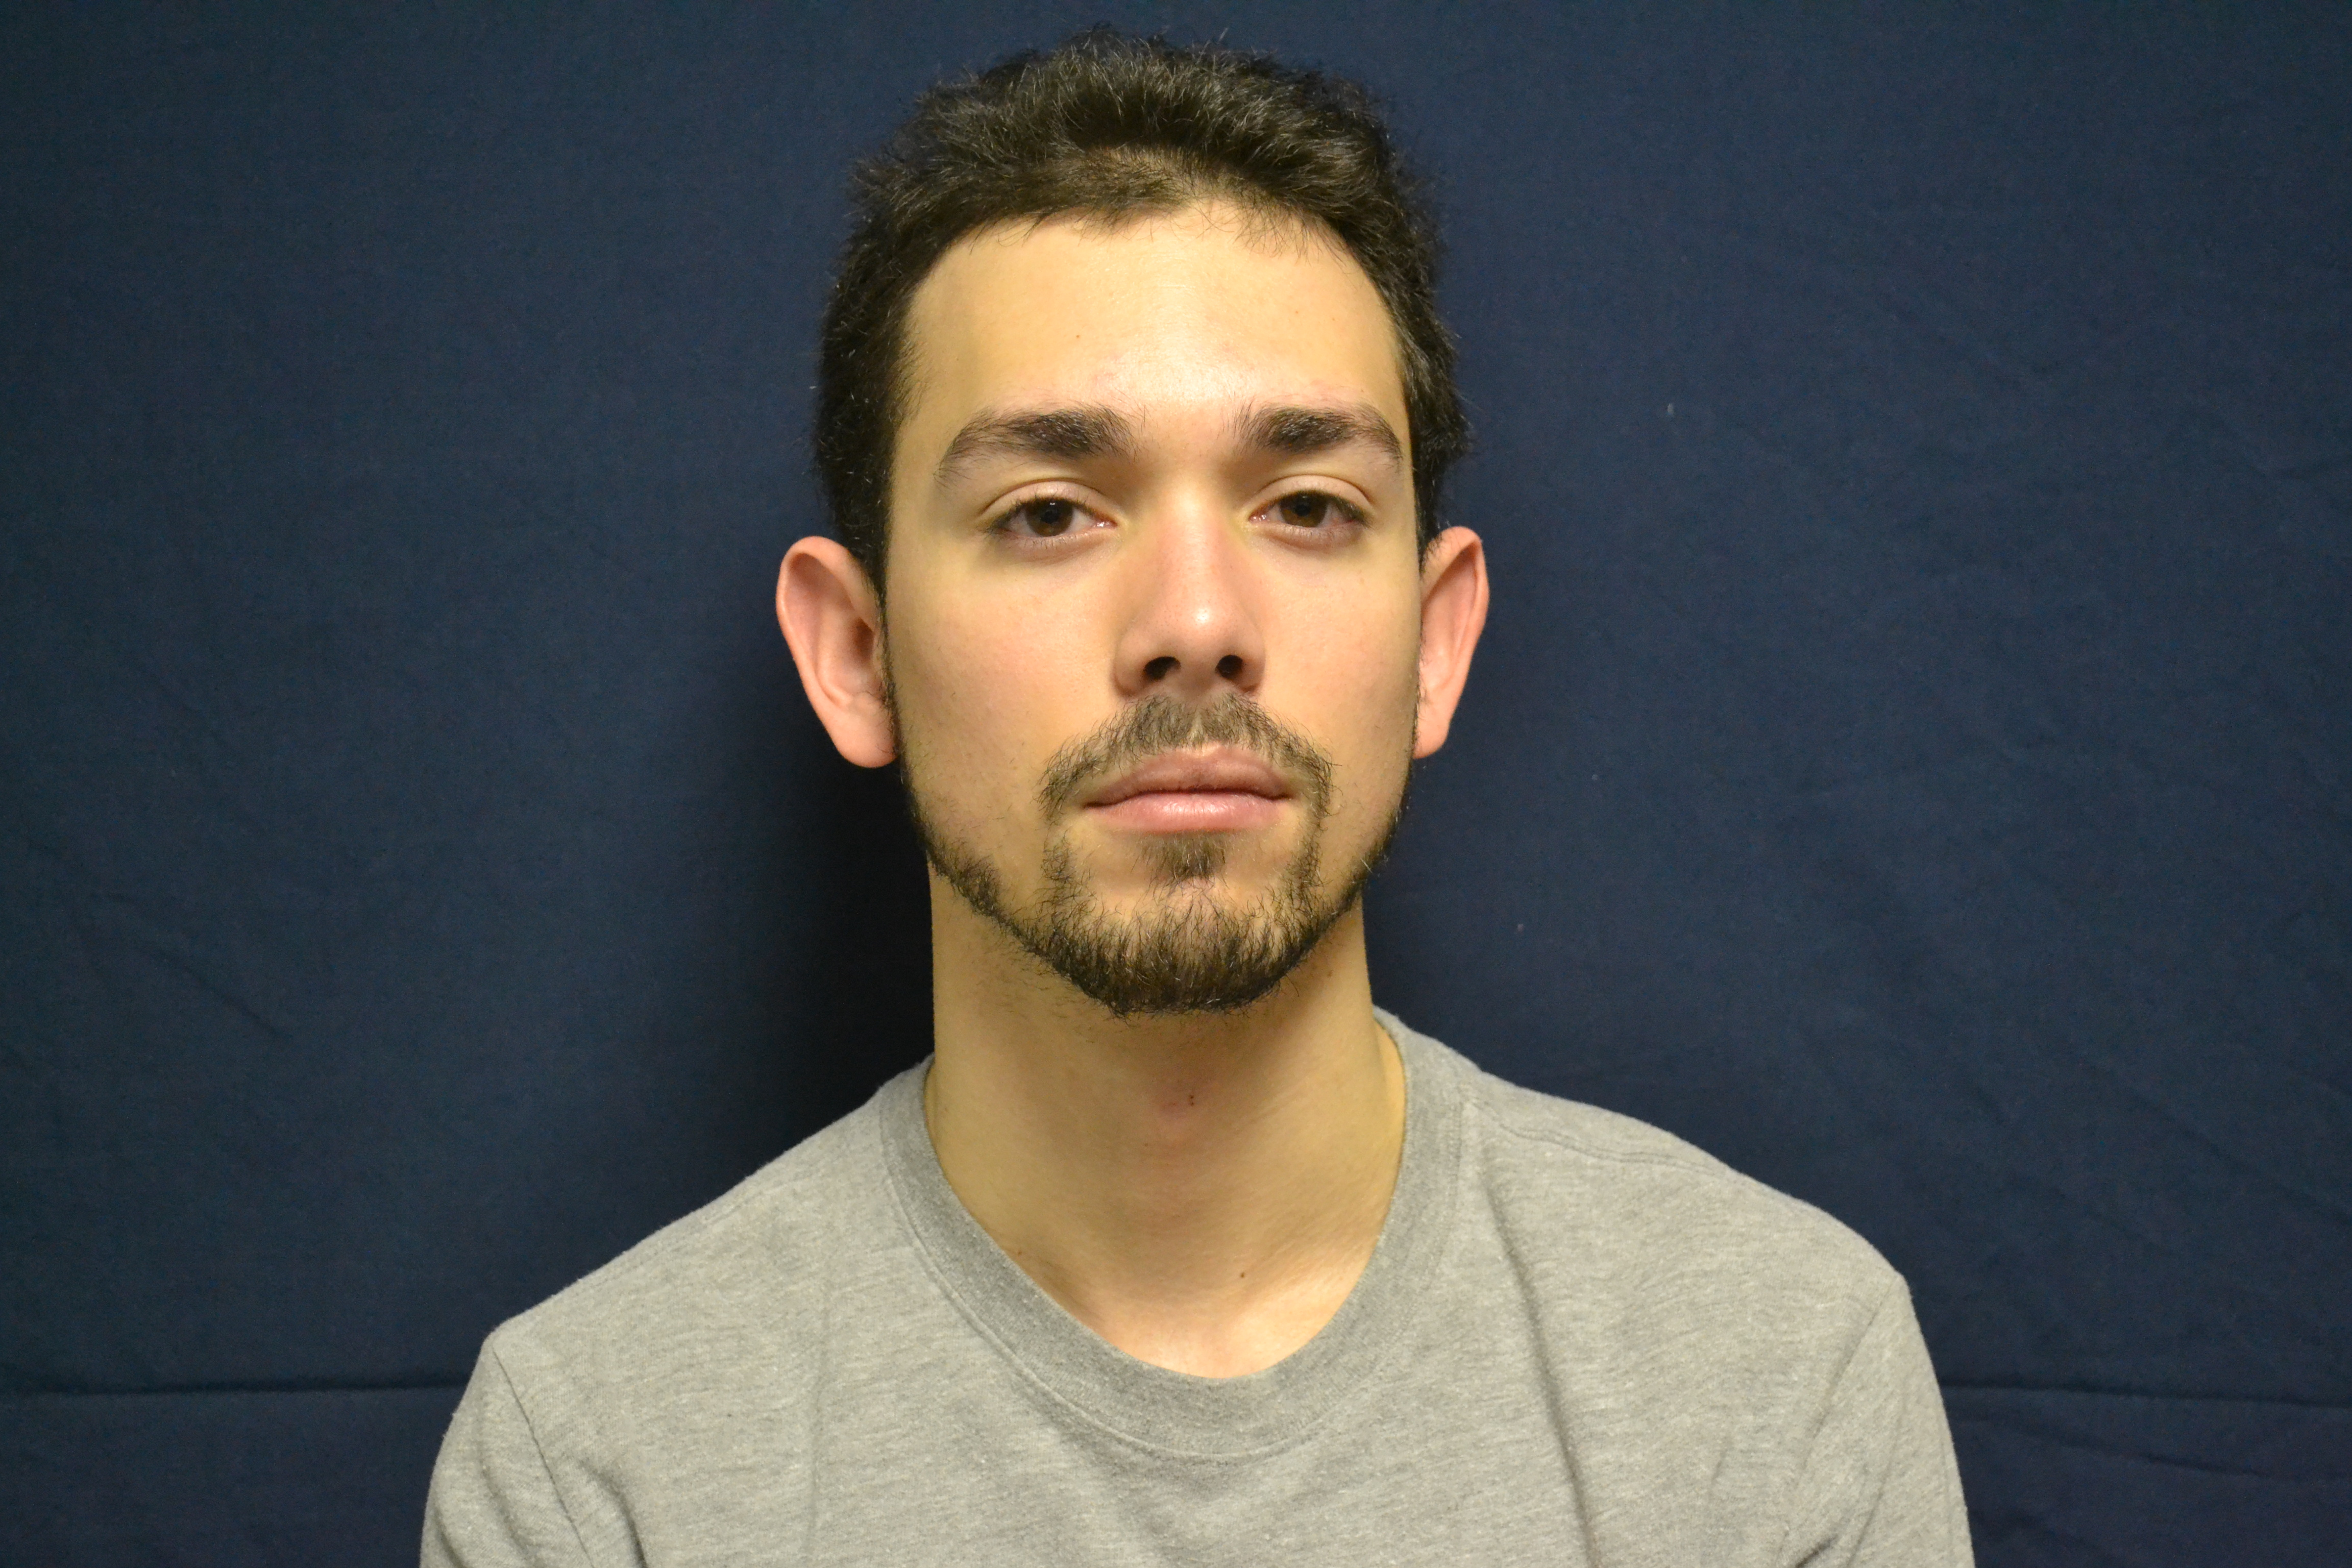
\includegraphics[scale = 0.15]{figures/ExcellentImg.jpg}
        \label{fig:excellentImg}\hspace{2cm}}
    \subfloat[Facial image with defects]
        {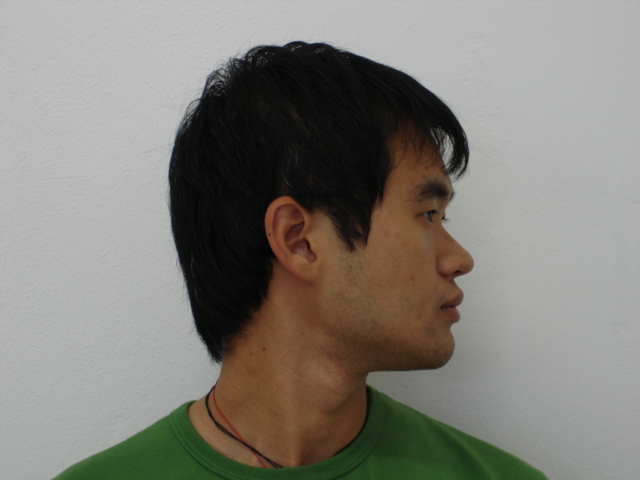
\includegraphics[scale = 0.23]{figures/FairImg.jpg}
        \label{fig:defectedImg}}
\end{figure}

Image \ref{fig:excellentImg} checks all bullet points 


\begin{figure}[H]
\centering
    \subfloat[Excellent facial image]
        {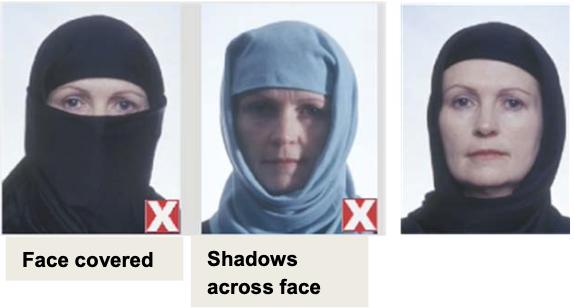
\includegraphics[scale = 0.65]{figures/FaceCovered.png}}
    \subfloat[Facial image with defects]
        {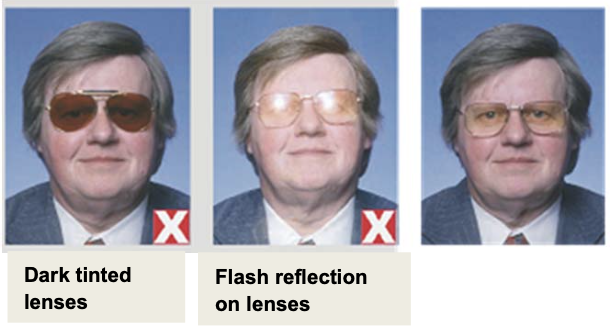
\includegraphics[scale = 0.65]{figures/SunglassesTinted.png}\hspace{3cm}}
        \vspace{0.5cm}
        \newline
    \subfloat[]
        {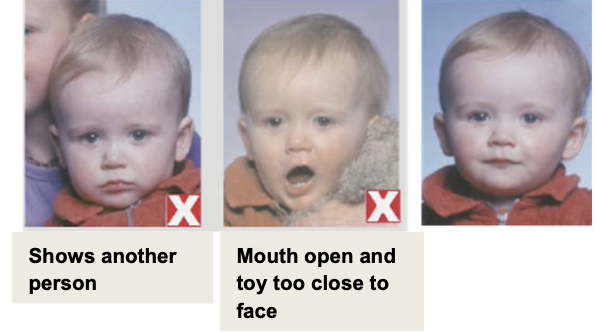
\includegraphics[scale = 0.65]{figures/BabyOpenMouth.png}}
\end{figure}


\section{Image quality metrics} 
Mobai chose the IQMs used in our application. The reason for choosing these specific metrics was their differences in terms of evaluating images of faces. 

Both metrics are open-source projects. 


\subsection{ISO metric}

\subsection{FaceQNet}
\chapter{Thesis Structure}

The structure of the thesis, i.e., which chapters and other document elements that should be included, depends on several factors such as the study level (bachelor, master, PhD), the type of project it describes (development, research, investigation, consulting), and the diversity (narrow, broad). Thus, there are no exact rules for how to do it, so whatever follows should be taken as guidelines only.

A thesis, like any book or report, can typically be divided into three parts: front matter, body matter, and back matter. Of these, the body matter is by far the most important one, and also the one that varies the most between thesis types.

\section{Front Matter}
\label{sec:frontmatter}

The front matter is everything that comes before the main part of the thesis. It is common to use roman page numbers for this part to indicate this. The minimum required front matter consists of a title page, abstract(s), and a table of contents. A more complete front matter, in a typical order, is as follows.

\begin{description}
    \item[Title page:] The title page should, at minimum, include the thesis title, authors and a date. A more complete title page would also include the name of the study programme, and possibly the thesis supervisor(s). See \cref{sec:setup}.
    \item[Abstracts:] The abstract should be an extremely condensed version of the thesis. Think one sentence with the main message from each of the chapters of the body matter as a starting point. \textcite{landes1951scrutiny} have given some very nice instructions on how to write a good abstract. A thesis from a Norwegian Univeristy should contain abstracts in both Norwegian and English irrespectively of the thesis language (typically with the thesis language coming first).
    \item[Dedication:] If you wish to dedicate the thesis to someone (increasingly common with increasing study level), you may add a separate page with a dedication here. Since a dedication is a personal statement, no template is given. Design it according to your preference.
    \item[Acknowledgements:] If there is someone who deserves a `thank you', you may add acknowledgements here. If so, make it an unnumbered chapter, i.e., \texttt{\textbackslash chapter*\{Acknowledgements\}}.
    \item[Table of contents:] A table of contents should always be present in a document at the size of a thesis. It is generated automatically using the \texttt{\textbackslash tableofcontents} command. The one generated by this document class also contains the front matter and unnumbered chapters.
    \item[List of figures:] If the thesis contains many figures that the reader might want to refer back to, a list of figures can be included here. It is generated using \texttt{\textbackslash listoffigures}.
    \item[List of tables:] If the thesis contains many tables that the reader might want to refer back to, a list of tables can be included here. It is generated using \texttt{\textbackslash listoftables}.
    \item[List of code listings:] If the thesis contains many code listings that the reader might want to refer back to, a list of code listings can be included here. It is generated using \texttt{\textbackslash lstlistoflistings}.
    \item[Other lists:] If there are other list you would like to include, this would be a good place. Examples could be lists of definitions, theorems, nomenclature, abbreviations, glossary etc. There are no standards for this, but many lists can be generated using the \texttt{description} environment (like, e.g., this list of possible front matter content) within a separate \texttt{\textbackslash chapter*\{\}}.
    \item[Preface or Foreword:] A preface or foreword is a good place to make other personal statements that do not fit whithin the body matter. This could be information about the circumstances of the thesis, your motivation for choosing it, or possibly information about an employer or an external company for which it has been written. Again, use, e.g., \texttt{\textbackslash chapter*\{Preface\}}.
\end{description}

\section{Body Matter}

The body matter consists of the main chapters of the thesis. It starts the Arabic page numbering with page~1. There is a great diversity in the structure chosen for different thesis types. Common to almost all is that the first chapter is an introduction, and that the last one is a conclusion followed by the bibliography.

\subsection{Development Project}
\label{sec:development}

For many bachelor and some master projects in computer science, the main task is to develop something, typically a software prototype, for an `employer' (e.g., an external company or a research group). A thesis describing such a project is typically structured as a software development report whith more or less the following chapters:

\begin{description}
    \item[Introduction:] The introduction of the thesis should take the reader all the way from the big picture and context of the project to the concrete task that has been solved in the thesis. A nice skeleton for a good introduction was given by \textcite{claerbout1991scrutiny}: \emph{review–claim–agenda}. In the review part, the background of the project is covered. This leads up to your claim, which is typically that some entity (software, device) or knowledge (research questions) is missing and sorely needed. The agenda part briefly summarises how your thesis contributes.
    \item[Requirements:] The requirements chapter should lead up to a concrete description of both the functional and non-functional requirements for whatever is to be developed at both a high level (use cases) and lower levels (low level use cases, requirements). If a classical waterfall development process is followed, this chapter is the product of the requirement phase. If a more agile model like, e.g., SCRUM is followed, the requirements will appear through the project as, e.g., the user stories developed in the sprint planning meetings.
    \item[Technical design:] The technical design chapter describes the big picture of the chosen solution. For a software development project, this would typically contain the system arcitechture (client-server, cloud, databases, networking, services etc.); both how it was solved, and, more importantly, why this architecture was chosen.
    \item[Development Process:] In this chapter, you should describe the process that was followed. It should cover the process model, why it was chosen, and how it was implemented, including tools for project management, documentation etc. Depending on how you write the other chapters, there may be good reasons to place this chapters somewhere else in the thesis.
    \item[Implementation:] Here you should describe the more technical details of the solution. Which tools were used (programming languages, libraries, IDEs, APIs, frameworks, etc.). It is a good idea to give some code examples. If class diagrams, database models etc. were not presented in the technical design chapter, they can be included here.
    \item[Deployment:] This chapter should describe how your solution can be deployed on the employer's system. It should include technical details on how to set it up, as well as discussions on choices made concerning scalability, maintenance, etc.
    \item[Testing and user feedback:] This chapter should describe how the system was tested during and after development. This would cover everything from unit testing to user testing; black-box vs. white-box; how it was done, what was learned from the testing, and what impact it had on the product and process.
    \item[Discussion:] Here you should discuss all aspect of your thesis and project. How did the process work? Which choices did you make, and what did you learn from it? What were the pros and cons? What would you have done differently if you were to undertake the same project over again, both in terms of process and product? What are the societal consequences of your work?
    \item[Conclusion:] The conclusion chapter is usually quite short – a paragraph or two – mainly summarising what was achieved in the project. It should answer the \emph{claim} part of the introduction. It should also say something about what comes next (`future work').
    \item[Bibliography:] The bibliography should be a list of quality-assured peer-reviewed published material that you have used throughout the work with your thesis. All items in the bibliography should be referenced in the text. The references should be correctly formatted depending on their type (book, journal article, conference publication, thesis etc.). If \texttt{biblatex} is correctly used as proposed by this template, the formatting will be taken care of automatically. The bibliography should not contain links to arbitrary dynamic web pages where the content is subject to change at any point of time. Such links, if necessary, should rather be included as footnotes throughout the document. The main point of the bibliography is to back up your claims with quality-assured material that future readers will actually be able to retrieve years ahead.
\end{description}

\subsection{Research Project}
\label{sec:resesarch}

For many master and some bachelor projects in computer science, the main task is to gain knew knowledge about something. A thesis describing such a project is typically structed as an extended form of a scientific paper, following the so-called IMRaD (Introduction, Method, Results, and Discussion) model:

\begin{description}
    \item[Introduction:] See \cref{sec:development}.
    \item[Background:] Research projects should always be based on previous research on the same and/or related topics. This should be described as a background to the thesis with adequate bibliographical references. If the material needed is too voluminous to fit nicely in the review part of the introduction, it can be presented in a separate background chapter.
    \item[Method:] The method chapter should describe in detail which activities you undertake to answer the research questions presented in the introduction, and why they were chosen. This includes detailed descriptions of experiments, surveys, computations, data analysis, statistical tests etc.
    \item[Results:] The results chapter should simply present the results of applying the methods presented in the method chapter without further ado. This chapter will typically contain many graphs, tables, etc. Sometimes it is natural to discuss the results as they are presented, combining them into a `Results and Discussion' chapter, but more often they are kept separate.
    \item[Discussion:] See \cref{sec:development}.
    \item[Conclusion:] See \cref{sec:development}.
    \item[Bibliography:] See \cref{sec:development}.
\end{description}



\section{Back Matter}

Material that does not fit elsewhere, but that you would still like to share with the readers, can be put in appendices. See \cref{app:additional}.

\input{chapters/4-conclusion.tex}

\chapter*{\bibname}
\printbibliography[heading=none]

\input{chapters/papers.tex}

\appendix
\input{appendices/a-appendix.tex}

\end{document}
